\documentclass[11pt]{article}
\usepackage{enumerate}
\usepackage{amsfonts}
\usepackage{graphicx}
\usepackage{tabularx}
\usepackage{pdflscape}

\pagestyle{empty} \setlength{\parindent}{0mm}
\addtolength{\topmargin}{-0.5in} \setlength{\textheight}{9in}
\addtolength{\textwidth}{1.75in} \addtolength{\oddsidemargin}{-0.9in}


\title{Sumerian Project\\
Software Requirements Specification\\
CS 491}
\author{Danielle Thurow \\
Seoung Jung\\
Zachary Fox\\
Thomas Fritchman}
\date{}


\begin{document}
\maketitle
\newpage

\tableofcontents
\newpage

\begin{center}
\Large Revision History\\
\begin{tabularx}{\textwidth}{|c|X|c|}
    \hline
    \textbf{Revision} & \textbf{Description} & \textbf{Date}\\ \hline
    1.0 & Initial Document & 6/6/2014\\ \hline
\end{tabularx}
\end{center}
\newpage

\section{INTRODUCTION}
\subsection{PURPOSE}
For assyriologists, consistently identifying months and years when the tablets were created is a vital part of recreating a Sumerian social network. The Date Extrapolator will solve this problem in two parts, and will be integrated with the work done by the previous group.\\

The first part is the implementation of an algorithm. This will identify the years and months, and will take into account things such as damage and scribes’ transcription errors. The conclusions of the algorithm will be tested against training data to analyse correctness. It will also accept outside input to attempt to correct any conclusions the algorithm has made. There will be a relatively easy way to adjust the parameters of the algorithm.\\

The second part of the solution is user interface. This will allow the user to give input on the algorithm’s correctness. It will also display statistics about the algorithm’s correctness.

\subsection{INTENDED AUDIENCE AND READING SUGGESTIONS}
Readers of this document include any persons involved in the development of this program as a whole. This document will outline all requirements necessary, pertaining to the Date Extrapolator program, and will create a bridge between the customer and designers, in order to create an agreement on what is crucial to the overall success of this project. 

\subsection{PRODUCT SCOPE}
\subsubsection{SCOPE OF INITIAL RELEASE}
\textbf{Release 1 will be:}\\
\textbf{FE-01} not implemented\\
\textbf{FE-02} not implemented\\
\textbf{FE-03} not implemented\\
\textbf{FE-04} implement way to tweak algorithm for our specific algorithm\\
\textbf{FE-05} basic web page that displays statistics information\\
\textbf{FE-06} A simple implementation of a semi-naive algorithm

\subsubsection{SCOPE OF SUBSEQUENT RELEASES}
\textbf{Release 2 will be:}\\
\textbf{FE-01} not implemented\\
\textbf{FE-02} provide web page that displays algorithmically-chosen dates from text for confirmation\\
\textbf{FE-03} adds confirmed dates to database and tweaks algorithm\\
\textbf{FE-04} no update\\
\textbf{FE-05FE-05} give the statistics a better GUI for web page\\
\textbf{FE-06} improve implementation/ statistics for our algorithm\\

\textbf{Release 3 will be:}\\
\textbf{FE-01} implement completely\\
\textbf{FE-02} tweak and improve\\
\textbf{FE-03 }tweak and improve\\
\textbf{FE-04} tweak and improve\\
\textbf{FE-05}  tweak and improve\\
\textbf{FE-06}  tweak and improve

\subsection{REFERENCES}
www.wwucuneiform.com\\
https://sites.google.com/site/wwucsseniorprojectcuneiform/

\section{OVERALL DESCRIPTION}
\subsection{PRODUCT PERSPECTIVE}
It is an extension of an existing project aiming to improve the functionality of the current software.

\subsection{CONTEXT DIAGRAM}
% GOOGLE DOC LOCATED AT  https://docs.google.com/drawings/d/1W66NcmfOpwPvw9OsoErPGBWN4S3hAmCVE3tXkCs0H8Y/edit?usp=sharing
\begin{center}
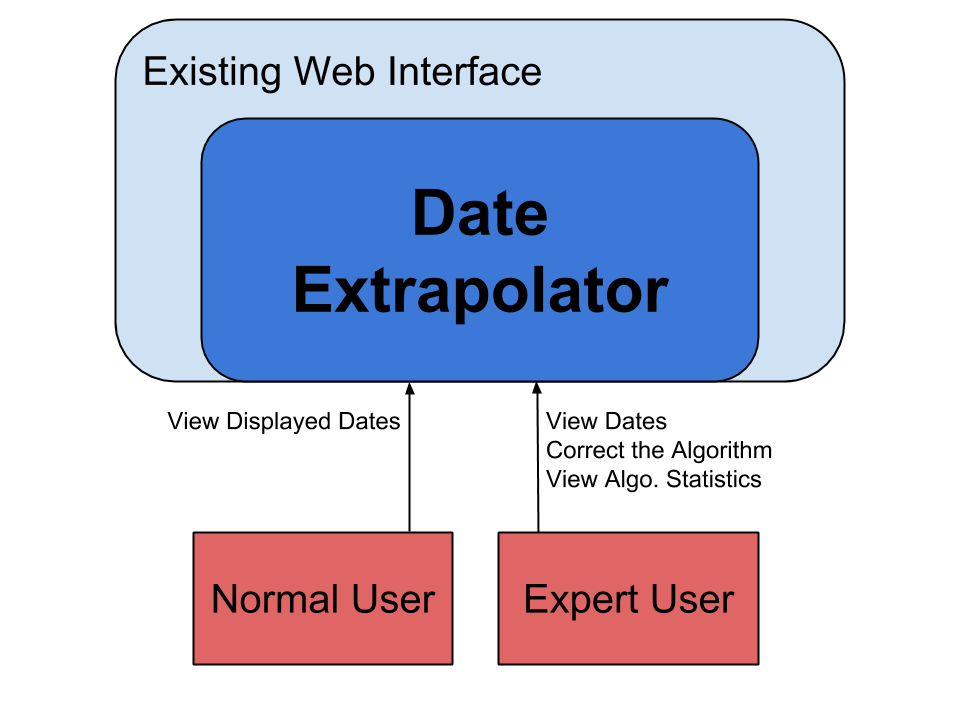
\includegraphics[scale=0.4]{ContextDiagram.png}
\end{center}

\subsection{USER CLASSES AND CHARACTERISTICS}
\begin{itemize}
    \item Expert User: an expert user is allowed to confirm or disagree with the algorithm’s suggested date, as well as do everything a normal user can.
    \item Normal user: A normal user is allowed to see the algorithm’s suggested dates and statistics of the current algorithm.
\end{itemize}

\subsection{OPERATING ENVIRONMENT}
This program is to be built into the currently existing web application.

\subsection{ASSUMPTIONS AND DEPENDENCIES}
\textbf{AS-1:} experts input is noncontroversial and correct
\textbf{AS-2:} there is enough time
\textbf{AS-3:} pattern exists in Sumerian date to create efficient algorithm

\textbf{DE-1:} depending on work of previous group’s work


\section{EXTERNAL INTERFACE REQUIREMENTS}
\subsection{USER INTERFACES}
Navigation controls will have a similar feel to the rest of the existing product.
UI details will be included in another specification.

\subsection{SOFTWARE INTERFACES}
PHP for website.\\
Java for database.\\
Python for cleaning the data.\\

\section{SYSTEM FEATURES}

\subsection{CORRECTIONAL INTERFACE}
\subsubsection{DESCRIPTION AND PRIORITY}
Allows expert users only to correct the dates the algorithm suggests.\\
Priority: High
\subsubsection{APPLICABLE USE CASES}
UC-02

\subsection{ALGORITHM TRAINING}
\subsubsection{DESCRIPTION AND PRIORITY}
Algorithm uses expert user’s input in order to refine itself. 
\subsubsection{APPLICABLE USE CASES}
UC-05\\
UC-02

\subsection{STATISTICS}
\subsubsection{DESCRIPTION AND PRIORITY}
Allows user to see the current statistics for the algorithm (such as correctness, parameters, etc.)
Priority: Medium
\subsubsection{APPLICABLE USE CASES}
UC-06\\
UC-01

\subsection{APPLIED ALGORITHM}
\subsubsection{DESCRIPTION AND PRIORITY}
Our current algorithm that will decide on dates in the tablets.\\
Priority: HIGH
\subsubsection{APPLICABLE USE CASES}
UC-04\\
UC-05

\section{OTHER NON-FUNCTIONAL REQUIREMENTS}
\subsection{PERFORMANCE REQUIREMENTS}
This application must calculate dates and display them to the user in a reasonable amount of time.
\subsection{SOFTWARE QUALITY ATTRIBUTES}
The top priority for the software quality is for it to be accurate 60\% of the time. It is designed to use the existing software already in place for this database. 
\subsection{USER DOCUMENTATION}
The user documentation will be minimal, the program should be intuitive enough that extra documentation is not required.
\subsection{PROJECT DOCUMENTATION}
We will include basic developer documentation for any continuation group after us.

\section{USE CASES}

% Use case table template
%\begin{tabularx}{\textwidth}{|l|X|X|X|}
%\hline
%\multicolumn{4}{|l|}{Name: }\\\hline
%Created By: & Group & Last Updated By: &  \\\hline
%Date Created: & 5/27/14 & Date Last Updated: &  \\\hline	
%\end{tabularx}
%
%\begin{tabularx}{\textwidth}{|l|X|}
%\hline
%Actor: & \\\hline
%Description: & \\\hline
%Preconditions: & \\\hline
%Postconditions: & \\\hline
%Priority: & \\\hline
%Frequency of Use: & \\\hline
%Normal Course of Events: & \\\hline
%Alternative Courses: & \\\hline
%Exceptions: & \\\hline
%Includes: & \\\hline
%Special Requirements: & \\\hline
%Assumptions: & \\\hline
%Notes and issues: & \\\hline
%\end{tabularx}

\begin{tabularx}{\textwidth}{|l|X|X|X|}
\hline
\multicolumn{4}{|l|}{Name: UC-01    Statistics Interface
}\\\hline
Created By: & Group & Last Updated By: &  \\\hline
Date Created: & 5/27/14 & Date Last Updated: &  \\\hline	
\end{tabularx}

\begin{tabularx}{\textwidth}{|l|X|}
\hline
Actor: & Expert user \\\hline
Description: & interface that allows user to view statistics\\\hline
Preconditions: & \\\hline
Postconditions: & \\\hline
Priority: & Medium \\\hline
Frequency of Use: & Medium/Low \\\hline
Normal Course of Events: & Go to tab/ link for statistics page\\\hline
Alternative Courses: & \\\hline
Exceptions: & \\\hline
Includes: & \\\hline
Special Requirements: & \\\hline
Assumptions: & \\\hline
Notes and issues: & \\\hline
\end{tabularx}
\newpage

\begin{tabularx}{\textwidth}{|l|X|X|X|}
\hline
\multicolumn{4}{|l|}{Name: UC-02    correct algorithm’s dates}\\\hline
Created By: & Group & Last Updated By: &  \\\hline
Date Created: & 5/27/14 & Date Last Updated: &  \\\hline	
\end{tabularx}

\begin{tabularx}{\textwidth}{|l|X|}
\hline
Actor: & Expert User\\\hline
Description: & interface that allows user to correct algorithm’s dates\\\hline
Preconditions: & must be identified as an expert user\\\hline
Postconditions: & algorithm needs to be corrected (UC-05)\\\hline
Priority: & Medium\\\hline
Frequency of Use: & roughly greater than 40\% of time\\\hline
Normal Course of Events: & Expert user clicks tab/link for correcting algorithm.
    Algorithm displays dates for tablet (UC-03).
    User corrects algorithm.
    Submits the changes
\\\hline
Alternative Courses: & \\\hline
Exceptions: & \\\hline
Includes: & UC-03\\\hline
Special Requirements: & \\\hline
Assumptions: & user is an expert\\\hline
Notes and issues: & \\\hline
\end{tabularx}
\newpage


\begin{tabularx}{\textwidth}{|l|X|X|X|}
\hline
\multicolumn{4}{|l|}{Name: UC-03    Display Dates}\\\hline
Created By: & Group & Last Updated By: &  \\\hline
Date Created: & 5/27/14 & Date Last Updated: &  \\\hline	
\end{tabularx}

\begin{tabularx}{\textwidth}{|l|X|}
\hline
Actor: & Expert user\\\hline
Description: & Interface that allows user to view the algorithm’s results\\\hline
Preconditions: & \\\hline
Postconditions: & \\\hline
Priority: & High\\\hline
Frequency of Use: & High\\\hline
Normal Course of Events: & User views tablet.
    Dates are displayed\\\hline
Alternative Courses: & \\\hline
Exceptions: & \\\hline
Includes: & \\\hline
Special Requirements: & \\\hline
Assumptions: & \\\hline
Notes and issues: & \\\hline
\end{tabularx}
\newpage

\begin{tabularx}{\textwidth}{|l|X|X|X|}
\hline
\multicolumn{4}{|l|}{Name: UC-04    process tablets}\\\hline
Created By: & Group & Last Updated By: &  \\\hline
Date Created: & 5/27/14 & Date Last Updated: &  \\\hline	
\end{tabularx}

\begin{tabularx}{\textwidth}{|l|X|}
\hline
Actor: & algorithm\\\hline
Description: & algorithm goes through tablets and identifies dates\\\hline
Preconditions: & tablet is in the database\\\hline
Postconditions: & \\\hline
Priority: & High\\\hline
Frequency of Use: & Every time expert user corrects algorithm\\\hline
Normal Course of Events: & Pull expert opinion (if any) (UC-05).
    Goes through database, dates them
\\\hline
Alternative Courses: & Pull expert opinion (if any) (UC-05)
    Only dates subset of database,\\\hline
Exceptions: & \\\hline
Includes: & UC-05\\\hline
Special Requirements: & \\\hline
Assumptions: & \\\hline
Notes and issues: & \\\hline
\end{tabularx}
\newpage

\begin{tabularx}{\textwidth}{|l|X|X|X|}
\hline
\multicolumn{4}{|l|}{Name: UC-05    pull expert opinion}\\\hline
Created By: & Group & Last Updated By: &  \\\hline
Date Created: & 5/27/14 & Date Last Updated: &  \\\hline	
\end{tabularx}

\begin{tabularx}{\textwidth}{|l|X|}
\hline
Actor: & algorithm\\\hline
Description: & algorithm gets expert user’s corrections\\\hline
Preconditions: & \\\hline
Postconditions: & \\\hline
Priority: & Medium\\\hline
Frequency of Use: & Every N time steps, pull expert user data from date extrapolator\\\hline
Normal Course of Events: & N time steps pass
    query date extrapolator for all expert user corrections\\\hline
Alternative Courses: & \\\hline
Exceptions: & \\\hline
Includes: & \\\hline
Special Requirements: & \\\hline
Assumptions: & \\\hline
Notes and issues: & \\\hline
\end{tabularx}
\newpage

\begin{tabularx}{\textwidth}{|l|X|X|X|}
\hline
\multicolumn{4}{|l|}{Name: UC-06    Algorithm Statistics}\\\hline
Created By: & Group & Last Updated By: &  \\\hline
Date Created: & 5/27/14 & Date Last Updated: &  \\\hline	
\end{tabularx}

\begin{tabularx}{\textwidth}{|l|X|}
\hline
Actor: & algorithm\\\hline
Description: & algorithm gives date extrapolator its current statistics\\\hline
Preconditions: & algorithm has run at least once\\\hline
Postconditions: & \\\hline
Priority: & Medium\\\hline
Frequency of Use: & Every time expert user queries about statistics\\\hline
Normal Course of Events: & Gets a query from date extrapolator (UC-03)
    gives current statistics to date extrapolator\\\hline
Alternative Courses: & \\\hline
Exceptions: & \\\hline
Includes: & UC-03\\\hline
Special Requirements: & \\\hline
Assumptions: & \\\hline
Notes and issues: & \\\hline
\end{tabularx}



\begin{landscape}
\begin{center}
\Large \textbf{Traceability Matrix}\\ 
\begin{tabular}{|m{2cm} |m{2.5cm}|m{2.5cm}|m{2.5cm}|m{2.5cm}|m{2.5cm}|m{2.5cm}|m{2.5cm}|}
	\hline
	& & \textbf{FE-01} & \textbf{FE-02} & \textbf{FE-03} & \textbf{FE-04}  & \textbf{FE-05} & \textbf{FE-06} \\ \hline
	&  & provide users ways to add new tablets
 & has interface which allows expert users to correct the algorithm results.
 & uses expert user’s input to update and refine algorithm.
 & a way to tweak algorithm 
  & show statistics for each algorithm
 & have an algorithm that pulls dates out of the tablets
 \\ \hline
	\textbf{UC-01} & Statistics Interface & &  &  &  & X &  \\ \hline
	\textbf{UC-02} & correct algorithm’s dates & &  & X & X &  & X \\ \hline
	\textbf{UC-03} & Display Dates & &  &  &  &  & X \\ \hline
	\textbf{UC-04} & process tablets & &  & X &  &  & X \\ \hline
	\textbf{UC-05} & pull expert opinion & & X &  &  &  &  \\ \hline
	\textbf{UC-06} & Algorithm Statistics & &  &  &  & X &  \\ \hline
\end{tabular}
\end{center}
\end{landscape}


\end{document}
